
% Inbuilt themes in beamer
\documentclass{beamer}
% Theme choice:
\usetheme{Madrid}

% Title page details: 
\title{Optimization in Energy and Power} 
\institute{IIT Hyderabad}

\begin{document}

\begin{frame}
    \titlepage 
    

\textbf{Group - 41}
\begin{itemize}
    \item{Kunal Nema - MA20BTECH11007}
    \item{Sparsh Gupta - MA20BTECH11015}
    \item{Varunaditya Singhal - MA20BTECH11021}
    \item{Prakhar Patni - MA20BTECH11014}
\end{itemize}

\end{frame}

\begin{frame}{Contents}
    \tableofcontents
\end{frame}

\section{Introduction}
\section{Vehicle Model}
\subsection{Battery Model}
\subsection{Road Load Model}
\subsection{Gearbox Model}
\subsection{Torque Split Model}
\subsection{Electric Motor Model}
\subsection{Engine Model}
\section{Problem Formulation}
\section{Iterative Algorithms}
\section{Results}
\section{Conclusion}





\begin{frame}{Introduction}
\begin{block}{ }
Applying optimization-based methods for the energy management of parallel hybrid vehicles to reach our desired optimal solution in less time.
\end{block}



\end{frame}
\begin{frame}{Introduction}
Few scenarios where convex optimization in Hybrid Electric Vehicle plays important role are:
\begin{itemize}
    \item \textbf{Inter-conversion:} Based on the parameter, if the driver himself wants to change the power source what parameters would be optimum to do so.
    \item \textbf{Battery boundaries:} When battery State of Charge reaches boundary condition then choosing optimum solution.
    \item \textbf{Destination:} Depending on the distance travelled and journey logistics the optimum fuel and battery consumption. 
\end{itemize}





\end{frame}

\begin{frame}{Vehicle Model}
    \begin{itemize}
        \item The Vehicle model conversion from non-linear vehicle model to approximated convex model.
        \item Expression of component model as convex optimization variables.
        \item Working with \textbf{3} decision variables i.e
        \begin{itemize}
            \item Engine on/off state.
            \item Torque spilt.
            \item Gear split.
        \end{itemize}
        \item Variable of our interest = Torque split.
    \end{itemize}
\end{frame}



\begin{frame}{Battery Model}

    \begin{block}{ }
        Formation of a convex model based on the figure , observing the open Voltage depending on SOC.
    \end{block}
        
        % \item 
    
    \begin{equation*}
   SOC(k + 1) = SOC(k) - \Delta t \cdot \frac{I_b(k)}{Q_0}
\end{equation*}
\begin{equation*}
   I_b(k) = \frac{V_{oc} −\sqrt{V_{oc}^2- 4 R_i(P_m(k)+P_{aux})}}{2 \cdot R_i} 
\end{equation*}
% \begin{itemize}
%     \item $I_b$ is the battery current.
%     \item $P_{aux}$ is a constant power consumed by electric auxiliary units.
%     \item $\Delta$ t is the sampling time = 1 sec.
% \end{itemize}
\end{frame}

\begin{frame}{Battery Model}
\begin{columns}
\begin{column}{0.45\textwidth}
   
    \begin{equation*}
  P_m(k) \leq V_{oc} \cdot I_b(k) − R_i \cdot I^2_b(k) − P_{aux} 
\end{equation*}
In order to maintain the convexity the variable of interest and battery SOC are being constraint as follows:
\begin{equation*}
  I_{b,min} \leq I_b(k) \leq I_{b,max} 
\end{equation*}
\begin{equation*}
  SOC_{min} \leq SOC(k) \leq SOC_{max} 
\end{equation*}
 \end{column}
\begin{column}{0.55\textwidth}
    \begin{figure}
    \centering
        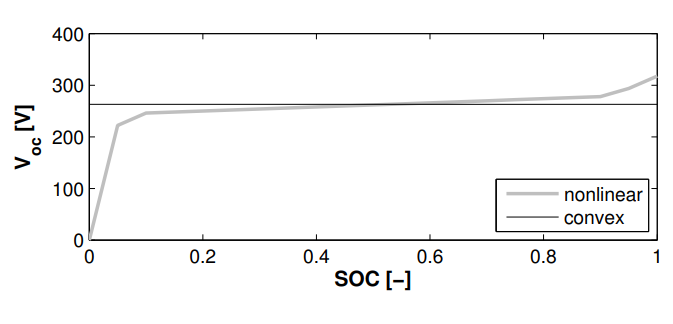
\includegraphics[width=0.7\textwidth, height=1\textwidth]{Voltage model .png}
        \caption{Open Voltage Model}
    \end{figure}
\end{column}
\end{columns}

\end{frame}


\begin{frame}{Road Load Model}
Let v(k) be speed of vehicle dependent on time k.

\begin{columns}
% Column 1
\begin{column}{0.5\textwidth}
\begin{itemize}
    \item Wheel Speed ($\omega_w$): \\ \begin{align*}
        \omega_w(k) = \frac{v(k)}{r_w}
    \end{align*}
    
    \item Wheel Torque ($T_w$): \\ \begin{align*}
T_w(k) = r_w \cdot \bigg\{\frac{1}{2}\rho_{air}c_d Av^2(k) + \\c_r m_v a_g  cos(\alpha(k)) + m_v a_g sin(\alpha(k))  + \\(m_v +m_r(g(k))) a(k)\bigg\}
\end{align*}
\end{itemize}

\end{column}
% Column 2    
\begin{column}{0.5\textwidth}
    \begin{figure}
    \centering
        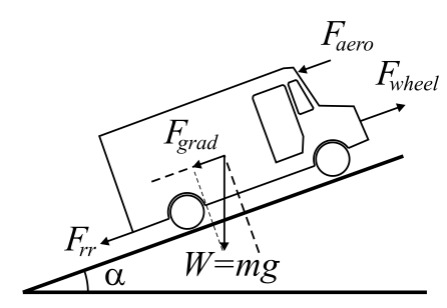
\includegraphics[width=0.7\textwidth]{road load model.jpeg}
        \caption{Road Load Model}
    \end{figure}
\end{column}
\end{columns}
    
\end{frame}


\begin{frame}{Gearbox Model}
Here $i_g$ represents gearbox ratio.

\begin{columns}
% Column 1
\begin{column}{0.5\textwidth}
\begin{itemize}
    \item Gearbox speed ($\omega_g$): \\ \begin{align*}
        \omega_g(k) = \omega_w(k) \cdot i_g(k)
    \end{align*}
    
    \item Gearbox Torque ($T_g$): \\ \begin{align*}
T_g(k) = T_w(k) \cdot \frac{1}{i_g(k)} \cdot \\{\bigg\{\eta_{g,0} - \frac{\eta_{g,1}}{\omega_{g,1} } \cdot \omega_g(k)\bigg\}^{-sign(T_w(k))}}
\end{align*}
\end{itemize}
    
\end{column}
% Column 2    
\begin{column}{0.5\textwidth}
    \begin{figure}
    \centering
        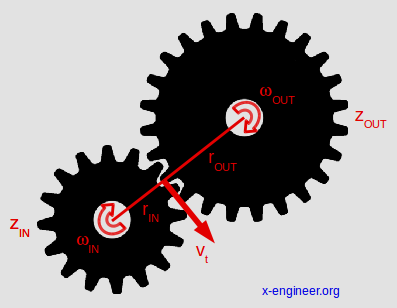
\includegraphics[width=0.7\textwidth]{gearbox model.png}
        \caption{Roadload to Gearbox}
    \end{figure}
\end{column}
\end{columns}

    
\end{frame}

\begin{frame}{Gearbox Model}
\begin{block}{ }
    Fuel consumption in Gear-shifting
\end{block}

\begin{itemize}
    \item   Equivalent fuel consumption per gearshift ($m_g$): \\ \begin{align*}
        m_g(k)= \begin{cases}
    0.01 & \text{if } g(k)\neq g(k-1)\\
    0              & \text{otherwise}
\end{cases}
    \end{align*}
    
    \item The gear g is being controlled by gear controlled variable ($u_g$): \\
    \begin{align*}
        g(k)= g(k-1) +u_g(k), \quad u_g \in \{-1,0,1\}
    \end{align*}
    
\end{itemize}
\end{frame}


\begin{frame}{Torque Split Model}
\begin{itemize}
    \item The torque split between the electric motor and the internal combustion engine is determined by the motor torque ($T_m$).
    
    \vspace{5pt}
    
    \item \begin{align*}
        T_e(k) = T_g(k) - T_{m}(k)
    \end{align*}
\end{itemize}
    
\end{frame}


\begin{frame}{Electric Motor Model}

\begin{columns}
% Column 1
\begin{column}{0.5\textwidth}
\begin{itemize}
    \item Motor Power ($P_m$): \\ \begin{align*}
        P_m \geq b_0(\omega_m) + b_1(\omega_m)T_m + b_2(\omega_m)T_m^2
    \end{align*}
    
    \item Convexity of the equation
    
    \item Limitation on motor speed:
    \begin{align*}
        0 \leq \omega_m(k) \leq \omega_{m,max}
    \end{align*}
    
    \item Limitation on motor torque:
    \begin{align*}
        T_{m,min}(\omega_m(k)) \leq T_m(k) \leq T_{m,max}(\omega_m(k))
    \end{align*}

\end{itemize}
\end{column}


% Column 2    
\begin{column}{0.5\textwidth}
    \begin{figure}
    \centering
        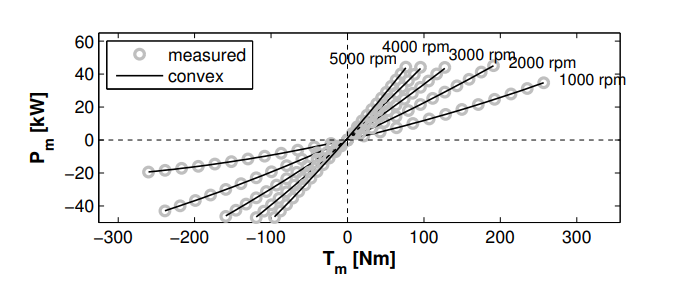
\includegraphics[width=0.75\textwidth, height=1\textwidth]{Electric Motor graph.png}
        \caption{Convex Motor Model}
    \end{figure}
\end{column}

\end{columns}
\end{frame}


\begin{frame}{Engine Model}
\begin{columns}
% Column 1
\begin{column}{0.5\textwidth}
\begin{itemize}
    \item Mass of fuel consumed ($\dot{\textit{\textbf{m}}}_f$)
    
    \item \begin{align*}
        \dot{\textit{\textbf{m}}}_f(k) \geq u_e(k)\cdot \bigg\{a_0&(k)+a_1(k)\cdot \\ \textbf{T}_e{k}+a_2(k)\cdot \textbf{T}_e^2(k)\bigg\}
    \end{align*}
    
    \item Convexity of the equation
    
    \item Limitation on engine speed:
    \begin{align*}
        \omega_{e,min} \leq \omega_e(k) \leq \omega_{e,max}
    \end{align*}
    
    \item Limitation on engine torque:
    \begin{align*}
        0 \leq T_e(k) \leq T_e(\omega_e(k))
    \end{align*}

\end{itemize}
\end{column}


% Column 2    
\begin{column}{0.5\textwidth}
    \begin{figure}
    \centering
        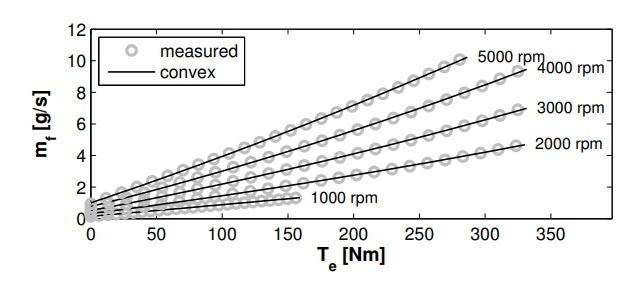
\includegraphics[width=0.7\textwidth, height=1\textwidth]{engine model.jpeg}
        \caption{Convex Engine Model}
    \end{figure}
\end{column}

\end{columns}
\end{frame}

\begin{frame}{Engine Model}
\begin{block}{ }
    Fuel consumption in change in state of engine.
\end{block}

\begin{itemize}
    \item The engine on/off decision is determined via the variable $u_e$ $\in$ \{0, 1\} such that the engine state (e) is
given by \\
\begin{align*}
    e(k) = u_{e}(k)
\end{align*}

    \item   Equivalent fuel consumption in changing state of engine ($m_e$): \\ \begin{align*}
    m_e(k)= \begin{cases}
    0.3 g & \text{if } e(k) = 1 \text{ and } e(k-1) = 0\\
    0              & \text{otherwise}
\end{cases}
    \end{align*}
    
\end{itemize}
\end{frame}




\begin{frame}{Problem Formulation}
\begin{itemize}
    \item The problem here for us is to minimize the overall fuel consumption, whenever the engine's running.
    \item We are dealing with 3 state variables here; Which are for,
    \begin{itemize}
        \item Engine On/off
        \item Gearshift
        \item State of Charge
    \end{itemize}
    \item We deal with Engine start and Gearshift through Dynamic Programming.
    \item For SOC optimization we use \emph{Convex Optimization}.
    
\end{itemize}
Note: We calculate the gearshift and engine On/Off variables in advance to solve the problem.  
\end{frame}

\begin{frame}{Problem Formulation}
    \begin{block}{Objective}
    Minimize:
    \[
        \sum_{k=1}^N \dot{\textbf{\textit{m}}}_f(k)\cdot \Delta t
    \]
    \end{block}
    \begin{itemize}
        \item The following objective depicts the fuel consumption which is being minimized by using the Electric power upon the intervals we are running the engine.
        \item Most of the constraints are derived on the basis of equations we had in Vehicle Model Description.
        \item Another constraint is the charge-sustenance condition which is-
        \begin{equation*}
            SOC(N+1) = SOC(1) = SOC_0
        \end{equation*}
        where $SOC_0$ is the initial SOC.   \end{itemize}
    
\end{frame}

\begin{frame}{Iterative Model}
    We begin by defining $s$ as our equivalence factor between fuel consumption and electrical energy. We find this equivalence factor by solving the aforementioned Convex Problem.
    
    \begin{figure}
        \centering
        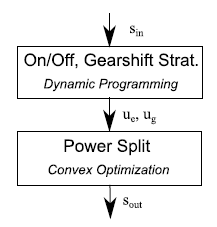
\includegraphics{Sequential.png}
        \caption{Sequential Model for Algorithm}
        \label{fig:seq}
    \end{figure}
\end{frame}

\begin{frame}{Iterative Model}
    \begin{block}{Optimality Condition}
        \centering
        $s_{out} \equiv s^*$ iff $s_{in} \equiv s_{out}$
    \end{block}
    
    
Keeping in mind the derived \emph{condition for optimality} we devise a iterative algorithm to find optimal values, starting off with a $s_{in}$ we begin our algorithm and iterate in the following way as shown in the upcoming slide.

\end{frame}

\begin{frame}{Iterative Model}
    \begin{figure}
    \centering
    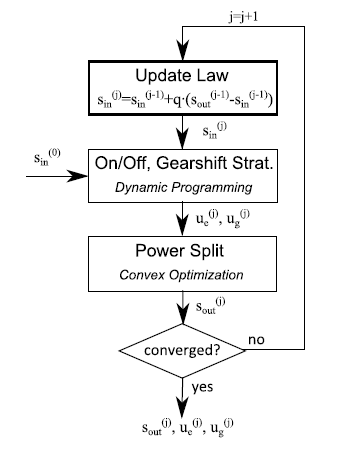
\includegraphics[scale=0.7]{Iterative.png}
    \caption{Iterations on Sequential Model}
    \label{fig:Iter}
    \end{figure}
\end{frame}

\begin{frame}{Iterative Model}

    \textbf{Steps in the Iterative model:}\\
    \begin{itemize}
        
    \item\textbf{Step 1: Initialization of the model}\\
    \begin{itemize}
        \item Includes initializing of the counter and equivalence factor.\\
    \end{itemize}
    \item\textbf{Step 2: Use of DP to obtain $u^{(j)}_g , u^{(j)}_e$}\\
    
    \begin{itemize}
        \item Values of $u^{(j)}_g$ and $u^{(j)}_e$ are obtained which are optimal for $s^{(j)}_{in}$ .
    \end{itemize}
    
    \item\textbf{Step 3: Use of convex optimization to obtain $s^{(j)}_{out}$}\\
        \begin{itemize}
            \item For the acquired values of $u^{(j)}_g$ and $u^{(j)}_e$ , we calculate the $s_{out}$.
        \end{itemize}
    
    \end{itemize}
    
\end{frame}

\begin{frame}{Iterative Model}
    \begin{itemize}
        \item\textbf{Step 4: Check for Convergence}\\
        \begin{itemize}
            \item  We calculate the root mean square error of the solution that we obtain for checking the tolerance of the solution using the following equation-
            \begin{equation*}
                E = \sqrt{\cfrac{1}{N}\sum_{k=1}^{N}(s_{in}(k)^{(j)} - s_{out}(k)^{(j)})^2}
            \end{equation*}
            \item If tolerance is higher than the tolerance level, increase j and update law as in step-5.
        \end{itemize}
    \end{itemize}
    

\end{frame}

\begin{frame}{Iterative model}
\begin{itemize}
    \item\textbf{Step 5: Update law}\\
    \begin{itemize}
        \item If Tolerance level is higher than the Maximum tolerance level, perform damping. We do the following update-
        \begin{equation*}
            s_{in}^{(j)} = s_{in}^{(j-1)} + q*(s_{out}^{(j-1)} - s_{in}^{(j-1)})
        \end{equation*}
        Here q is initialized at 0.2 and whenever the error is high we set $q \rightarrow 0.7.q$\\
        Using this law $s_{out}$ converges to the optimal solution.
        
    \end{itemize}
    
\end{itemize}
    
\end{frame}

\begin{frame}{Result}
    \begin{itemize}
        \item The minimum and maximum values of the SOC are assumed to be 20\% and 80\%, respectively.
        \item The given table summarizes the fuel consumption, the number of engine starts, the number of gearshifts, and the 
        computation time for the four cases considered-


        \item Summarizing the findings described in this section, the DP-C method yields more accurate results in much less time than a pure DP implementation.
    \end{itemize}
\end{frame}

\begin{frame}{Results}
\begin{figure}
    \centering
    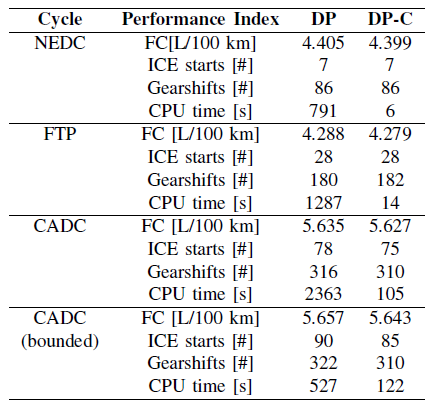
\includegraphics[scale=0.7]{Results.png}
    \caption{Comparison}
    \label{fig:Tab}
\end{figure}
    
\end{frame}

\begin{frame}{Conclusion}
\begin{itemize}
    \item This paper presents a method to calculate the globally optimal energy management strategy for a parallel HEV on a given driving cycle taking into account penalties to avoid frequent engine start and/or gearshift events. 
    \item The proposed method can be extended to other vehicle topologies and different formulations of the energy management problem
    
\end{itemize}

\end{frame}

\begin{frame}{Optimization in Energy and Power}
 \begin{center}
   \textbf{THANK YOU} \\
    \vspace{0.5cm}
    Group - 41\\
    \vspace{1cm}

 \end{center}   
    
\end{frame}


\end{document}